\documentclass{standalone}

\begin{document}

\section[Dataset]{CHIMeRA datasets}\label{chimera:net}

We have seen how we can extract useful information also from unstructured databases using a \textsf{web-scraping} pipeline.
The \emph{on-line doctor} web pages could be very useful for a toy model application like the \textsf{SymptomsNet}, but if we want to produce scientific relevant results, we have to take care about the validity of data.
Since English dataset availability is easier than the Italian one, we moved to more \quotes{robust} databases.

As told in the previous sections, there are a lot of studies performed on disease associations to other biomedical agents and in many cases the resulting datasets are publicly available on Internet.
This is the case of DisGeNET~\cite{DisGeNet} and DrugBank~\cite{DrugBank} datasets, which contain relationships between a large number of diseases with genes/variants (SNPs) and drugs (and other information), respectively.
DisGenet \href{https://doi.org/10.1093/nar/gkw943}{web-page} allows to download the datasets already stored into a well structured network format (sparse adjacency matrix, with \numprint{210498} associations between \numprint{117337} SNPs, \numprint{10358} diseases and \numprint{17549} genes), while DrugBank poses more issues to the treatment of data: DrugBank was designed to provide a large set of information related to each drug, using its own website and thus it needs a huge pre-processing of the JSON dataset structure to highlight all the possible network associations (\numprint{14812} drugs, \numprint{649} metabolite pathways, \numprint{3256} gene targets, \numprint{40} SNP targets, and \numprint{532} food interactions).
Using DisGenet we can connect diseases to their related genes and variants.
From the reviewed format of DrugBank, instead, we can link each disease to the associated drugs.
Associated to each drug we have also a list of gene and SNP targets, which can be merged to the information provided by DisGenet.
Moreover, we can insert also food interactions, metabolite pathways and drug interactions (synergy or not) extracted from DrugBank.
We would stress that, despite the trivial overlaps between the same data types (genes, diseases and SNPs up to now), just using the rearrangement of these pair of databases into a network structure, we can already provide a possible extrapolation of the underlying information, using the paths between nodes.
Starting from a disease inside DisGenet, using a single-database approach we can study \quotes{causality} relationships with the connected genes or SNPs.
Using a multiple-databases (or a network-of-networks structure) approach, we can map that disease to other kinds of information like drugs, foods and metabolite pathways.
The aim of such a network-of-networks structure is to unveil relationships hidden by the underwhelming overlap between single-type information across different databases.
The set of different information merged can thus be exploited for applications such as wide-scale drug effect evaluation and design, addressing general diagnostic questions for systems medicine and diseases etiology expansion.
In other words, a network-of-networks structure allows the inference of missing connections using node contraction.
A full list of the information collected by our \textsf{web-scraping} and rearrangement pipelines into the \textsf{CHIMeRA} database is shown in Tab.~\ref{tab:chimera_db}.

To enlarge our disease information we looked for other on-line data sources.
A very interesting database is given by HMDB~\cite{HMDB} (\emph{Human Metabolite Data Bank}), which comprises a vast amount of metabolites and metabolite-pathways with the associated drugs and diseases (\numprint{114003} metabolite entries, with chemical taxonomies and $\sim$\numprint{25000} human metabolic and disease pathways\footnote{
  The human metabolite-pathways can be divided into different types according to the informations stored in the HMDB dataset.
  The interactions between HMDB and DrugBank was already established through a vast series of hyper-links which connect them using metabolites and metabolite-pathways information.
  In this way we mapped also the information related to metabolite-pathways types to DrugBank dataset, obtaining a finer grain nomenclature and classification of these data.
  These informations can be used to improve our disease information.
  In Tab.\ref{tab:chimera_db} is shown only the aggregated data.
}).
The interconnections with the previous discussed datasets are straightforward, but in this case the data are not publicly available and we needed to apply a \textsf{web-scraping} algorithm to get its information.
An analogous procedure was applied to extract the data stored into \href{https://www.rxlist.com/script/main/hp.asp}{RXList} database.
RXList is an on-line website very similar to the previous discussed auto-diagnosis tools, where we can find associations between diseases, drugs and other several pathogenic associations.
In this case we have a further distinction between diseases: we have diseases related to drugs and diseases connected to other caused-diseases.
We have taken care of this kind of association using directional links\footnote{
  For sake of clarity, we encountered the same discrimination also into DrugBank dataset, in which we had intra-drug connections related to synergies or not in the use of multiple drugs together.
}.
We remark that each \textsf{web-scraping} pipeline has been customized according to a precise website, so for each analyzed case a different code has been developed to address the data extraction.

All these information can enrich our database and the description of a given disease, but we have to face the problem of data merging.
As previously discussed, we do not have a unique nomenclature for diseases and we can find analogous names (periphrases or synonyms) which identify the same concept (disease).
A useful tool to overcome these issues is given by a synonym dictionary: a powerful example is the CTD~\cite{CTDdb} (\emph{Comparative Toxicogenomics Database}, \numprint{7212} diseases with mapped synonyms and \numprint{4340} diseases with related phenotypes) database.
Using CTD jointly with SNAP~\cite{biosnapnets} (\emph{Stanford Large Network Dataset Collection}, \numprint{8803} disease terms with related synonyms) database we could enlarge the number of synonyms associated to each disease name.

\begin{table}
\hspace{-2cm}
\begin{tabular}{lcccccccc}
\hline\rowcolor{darkgrayrow}
                        & disease             & drug     & food     & gene     & metabolite & phenotype & SNP      & metabolic \\
\rowcolor{darkgrayrow}
                        &                     &          &          &          &            &           &          & pathway   \\
disease                 & CTD                 & RXList   &    x     & DisGeNET &  HMDB      & CTD       & DisGeNET & HMDB      \\
                        & RXList              &          &          &          &            &           &          &           \\
                        & SNAP                &          &          &          &            &           &          &           \\
drug                    &       RXList        & DrugBank & DrugBank &    x     &    x       &    x      &     x    & DrugBank  \\
food                    &          x          & DrugBank &    x     &    x     &    x       &    x      &     x    &    x      \\
gene                    &      DisGeNET       &    x     &    x     &    x     &    x       &    x      &     x    &    x      \\
metabolite              &       HMDB          &    x     &    x     &    x     &    x       &    x      &     x    & HMDB      \\
phenotype               &        CTD          &    x     &    x     &    x     &    x       &    x      &     x    &    x      \\
SNP                     &      DisGeNET       &    x     &    x     &    x     &    x       &    x      &     x    &    x      \\
metabolic               &        HMDB         & DrugBank &    x     &    x     &  HMDB      &    x      &     x    &    x      \\
pathway                 &                     &          &          &          &            &           &          &           \\
\hline\\
\# nodes                &  63974              & 35161    & 532      & 18799    &  114100    & 13214     & 117337   &  1329     \\
\hline\\
\end{tabular}
\caption{Description of the data mined by the \textsf{CHIMeRA} project before merging.
The datasets were collected using custom web-scraping pipelines and by a rearrangement of the public data.
For each pair of data types we report the list of datasets used to evaluate the interaction.
}
\label{tab:chimera_db}
\end{table}

We remember that the crucial point of our merging procedure is given by disease nodes, since they are the node type shared along (almost) all the databases.
The help given by synonym dictionaries increases the overlap between the mined datasets, but we chose to maximize it using a further NLP pipeline.
We began our pipeline using a word \emph{standardization}, i.e converting all words into their lower case formats and replacing all punctuation characters with a unique one\footnote{
  An unexpected issue arise in this step: different databases use different enumeration system.
  In some entries we found disease names associated to numbers which identify their multiple types.
  An example could be \quotes{Polyendocrine Autoimmune Syndrome type 1} but at the same time in a second database the same disease could be represented by \quotes{polyendocrine autoimmune TYPE I}.
  Despite the global differences between the two names, given in this case by upper- and lower-cases of some letters and the deletion of some words, a very critical odds is the enumeration style.
  The performances of our pipeline dramatically increased using a \textsf{roman\_number\_converter} algorithm.
}.
Then, we noticed that a not negligible part of words involved into disease names was useless for the description: words like \quotes{syndrome}, \quotes{disease}, \quotes{disorder}, \quotes{deficiency}, $\cdots$ are not informative and they can be ignored (filtered).
Then, we split disease names into a series of token according to the list of words which compose them (\emph{tokenization}) and sort them.

To further increase the overlap we transformed inflected words to their root form, using a \emph{stemming} algorithm: the stemmer strength has to be tuned according to the desired result.
A first processing was performed using a \textsf{Lancaster} stemmer (more aggressive).
If the resulting output was too short to be compared with other names, the starting token was processed by a \textsf{Porter Snowball} stemmer (less aggressive).
The choice of stemmer algorithm is a very crucial task for NLP, because, using it, we irreversibly loose information.
Other processing steps were performed for critical cases encountered during the analysis: these steps constrain our pipeline and they tuned it for the underlying application.

The work-flow output includes multiple false-positive matches: the pipeline performs a brute force processing and some information lost along the steps could be significants.
These cases lead to having multiple processed (same) names belonging to several (different) diseases: an example is shown in Fig.~\ref{fig:chimera_pipe}.
Considering the original name and the processed one (pipeline output), we merged two names using a score match.
This can be achieved introducing the standard word metrics: a common distance between words can be evaluated using the \emph{Levenshtein Distance} which follows the equation

$$
d_{a, b}(i, j) = \left\{ \begin{array}{rc}
  \max(i, j)                                                       & \mbox{if   } \min(i, j) = 0 \\
  \mbox{min} \left\{ \begin{array}{r}
      d_{a, b}(i - 1, j) + 1                     \\
      d_{a, b}(i, j - 1) + 1                     \\
      d_{a, b}(i - 1, j - 1) + 1_{(a \neq b)}    \\
    \end{array}
    \right.                                                        & \mbox{otherwise}            \\

  \end{array}
  \right.
$$
\\
where $a$ and $b$ are two strings of length $|a|$ and $|b|$ respectively.
The \emph{indicator function} $1_{(a \neq b)}$ is equal to $0$ when $a_i = b_j$ and $1$ otherwise.
In this way the Levenshtein distance between $a$ and $b$ evaluates the distance between the first $i$ characters of $a$ and the first $j$ characters of $b$.
Despite the apparently complexity of the mathematical equation, the \emph{Levenshtein Distance} is a particular case of the more general \emph{Edit Distance}, i.e a way to quantifying how dissimilar two strings are to one another by counting the minimum number of operations required to transform one string into the other.
Also in this case an example could be more explanatory: given the two strings \quotes{\emph{kitten}} and \quotes{\emph{sitting}}, their \emph{Levenshtein distance} is equal to $3$, in fact

\begin{enumerate}

  \item \textbf{k}itten $\rightarrow$ \textbf{s}itten (substitute \quotes{s} for \quotes{k})
  \item sitt\textbf{e}n $\rightarrow$ sitt\textbf{i}n (substitute \quotes{i} for \quotes{e})
  \item sittin $\rightarrow$ sittin\textbf{g} (insert \quotes{g} at the end)

\end{enumerate}

Using the Levenshtein formula we evaluated the distances between two original names and we associated the disease to the higher scorer.
A summary scheme of our pipeline is shown in Fig.~\ref{fig:chimera_pipe}.

\begin{figure}[htbp]
\centering
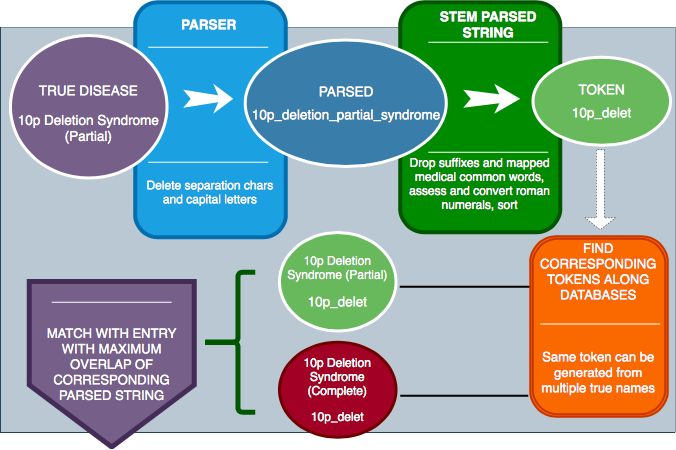
\includegraphics[width=\linewidth]{chimera_pipeline.png}
\caption{Scheme of the NLP pipeline developed in the \textsf{CHIMeRA} project.
The disease words are processed in multiple step as showed in the example.
}
\label{fig:chimera_pipe}
\end{figure}

The described NLP pipeline further increases the database overlaps (e.g CTD-SNAP 24.17\%; DisGenet-RXList 19.78\%).
We manually supervised the merging procedure taking care to reduce the false positive percentage.
In some cases, the overlap percentage remained low also after the application of our pipeline (e.g. RXList-HMDB 8.03\%; SNAP-HMDB 0.39\%).
Different data sources could be focused on different types of information and it is therefore reasonable to assume that, in some cases, the overlap is low.
We supervised these critical cases with a manual check and we demonstrated our hypothesis.
This behavior supports our databases choice: they include complementary information, which could improve the informative power of our structure.
At the same time, this result also proved the efficiency of our pipeline, confirming that the union of multiple data sources could effectively enlarge our knowledge about biomedical agents.

\begin{figure}[htbp]
\centering
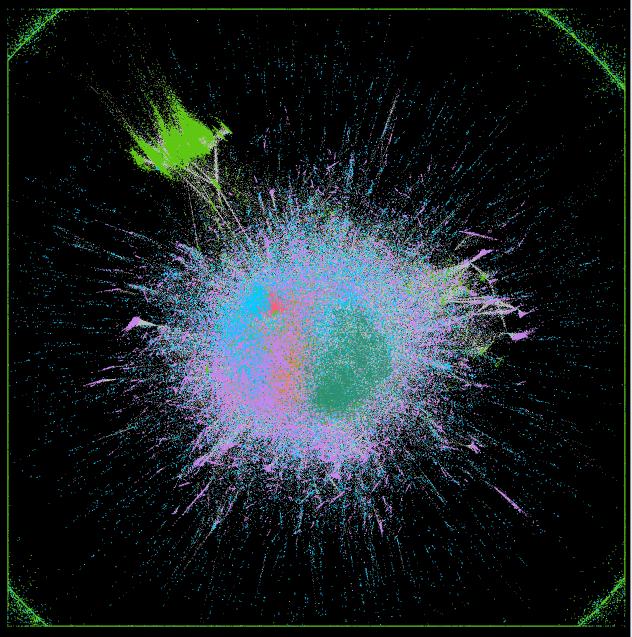
\includegraphics[width=\linewidth]{chimera_plot.png}
\caption{Graphical rendering of the first version of \textsf{CHIMeRA} network.
The visualization was performed before the inclusion of DrugBank dataset.
For computational issues we have not performed newer image of the global structure.
In the image we represented disease nodes (azure), gene nodes (orange), SNP nodes (purple), metabolite nodes (light green), drug nodes (pink) and phenotype nodes (dark green).
The visualization was obtained by the \emph{Atlas layout} provided by \textsf{Gephi}.
}
\label{fig:chimera}
\end{figure}

The output of our merging procedure allows the realization of the \textsf{CHIMeRA} network, i.e a network with more than $3.6\times10^5$ nodes and more than $3.8\times10^7$ links (ref. Fig.\ref{fig:chimera}).
In our resulting structure we have $7$ node types: disease (\numprint{63974}), drug (\numprint{35161}), gene (\numprint{18799}), SNP (\numprint{117337}), metabolite (\numprint{114100}), phenotype (\numprint{13214}), metabolite-pathway (\numprint{1329}) and food (532).
The full network adjacency matrix is still a block matrix, i.e we have not all the combinations of information in our database.
An emblematic case is given by food nodes: we have food information only into DrugBank and thus they would be connected only with drug types.
On the other hand, our network architecture could be easily improved adding new data sources: food nodes are pendant nodes that could be easily connected to other kinds of data, introducing new node types or just filling the available blocks.
\textsf{CHIMeRA} is still a work in progress project so we are still looking for improvements and new databases to add.

% disease= 63974
% drug= 35161
% gene= 18799
% SNP= 117337
% metabolite= 114100
% phenotype= 13214
% metapathway= 1329
% food= 532

% total= 364446

\end{document}
